\documentclass[letterpaper, 11pt]{article}
%\usepackage[hmargin = 1in, vmargin = 1in]{geometry}
\usepackage{amsmath}
\usepackage{amssymb}
\usepackage{enumitem}
\usepackage{mathrsfs}
\usepackage{tikz}
\usepackage{graphicx}
\usepackage{algorithmicx}
\usepackage{algpseudocode}
\setlength{\headheight}{14pt}
\usepackage{fancyhdr}
\pagestyle{fancy}
\rhead{Gabriel Wallace}
\lhead{Comp Sci 4250}

\usepackage{hyperref}
\hypersetup{
    colorlinks=true,
    linkcolor=blue,
    filecolor=magenta,      
    urlcolor=blue
}

\newcommand{\hwnumber}[1]{\medskip \noindent\textbf{#1.} \smallskip}

\begin{document}
\begin{center}
	{\LARGE Project 3}\\
\end{center}

The source code for this project can be found 
\href{https://github.com/gwallace04/cs4250/blob/311e0a3d9632a4600a3897c03d33dc0fb7f74519/proj3.txt}{here.}

\hwnumber{1} 

Queries and output of part 1:
\begin{enumerate}[label=(\alph*)]
	\item \texttt{?- parent\_of(pete, mark).} \\ true 
	\item \texttt{?- parent\_of(anne, jenny).} \\ false 
	\item \texttt{?- father\_of(X, todd).} \\ X = matt
	\item \texttt{?- sibling(X, tom).} \\ X = mark \\ X = anne
	\item \texttt{?- brother\_of(X, lilly).} \\ X = john \\ X = frank
	\item \texttt{?- grandparent\_of(X, henry).} \\ X = anne
	\item \texttt{?- sister\_of(X, alice).} \\ false
	\item \texttt{?- brother\_of(frank, kate).} \\ false
	\item \texttt{?- mother\_of(X, matt).} \\ X = anne
	\item \texttt{?- brother\_of(mark, anne).} \\ true
\end{enumerate}

\newpage

\hwnumber{2}

The output (with tracing) for the first call can be found in figure \ref{fig:one} and
the output (without tracing) for the second call can be found in figure \ref{fig:two}.

\begin{figure}[h]
	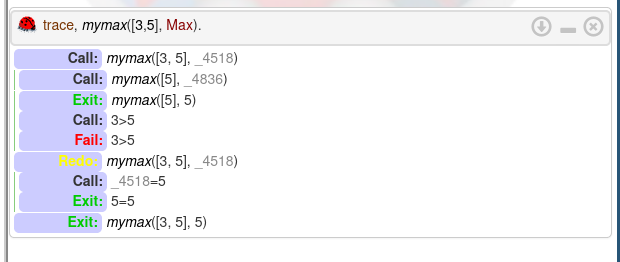
\includegraphics[width=\linewidth]{proj3_q2.png}
	\centering
	\caption{First call}
	\label{fig:one}
\end{figure}
\begin{figure}[h]
	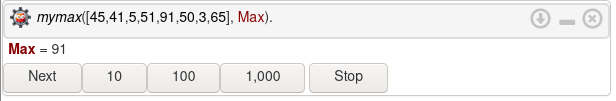
\includegraphics[width=\linewidth]{proj3_q2B.png}
	\centering
	\caption{Second call}
	\label{fig:two}
\end{figure}

\newpage
\hwnumber{3}

Output for the code can be found in figure \ref{fig:third}. 
\begin{figure}[h]
	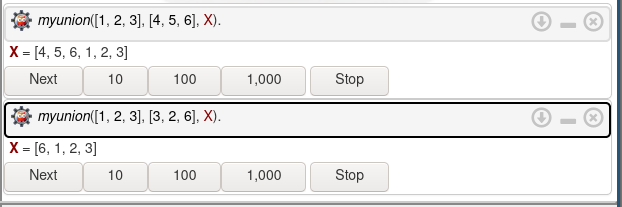
\includegraphics[width=\linewidth]{proj3_q3.png}
	\centering
	\caption{Part 3}
	\label{fig:third}
\end{figure}


\end{document}
